% The comment below tells Rubber to compile the .dot files.
%
% rubber: module graphics
% rubber: rules rules.ini

\documentclass{beamer}

\usetheme{default}

\usefonttheme{structurebold}
\usepackage{helvet}
\usecolortheme{seagull}         % white on black

\usepackage[utf8]{inputenc}
\PassOptionsToPackage{hyphens}{url}\usepackage{hyperref,xspace,multicol}
\usepackage[absolute,overlay]{textpos}
\usepackage{tikz}
\usetikzlibrary{arrows,shapes,trees,shadows,positioning}
\usepackage{fancyvrb}           % for '\Verb'
\usepackage{xifthen}            % for '\isempty'

% Remember the position of every picture.
\tikzstyle{every picture}+=[remember picture]

\tikzset{onslide/.code args={<#1>#2}{%
  \only<#1>{\pgfkeysalso{#2}} % \pgfkeysalso doesn't change the path
}}

% Colors.
\definecolor{guixred1}{RGB}{226,0,38}  % red P
\definecolor{guixorange1}{RGB}{243,154,38}  % guixorange P
\definecolor{guixyellow}{RGB}{254,205,27}  % guixyellow P
\definecolor{guixred2}{RGB}{230,68,57}  % red S
\definecolor{guixred3}{RGB}{115,34,27}  % dark red
\definecolor{guixorange2}{RGB}{236,117,40}  % guixorange S
\definecolor{guixtaupe}{RGB}{134,113,127} % guixtaupe S
\definecolor{guixgrey}{RGB}{91,94,111} % guixgrey S
\definecolor{guixdarkgrey}{RGB}{46,47,55} % guixdarkgrey S
\definecolor{guixblue1}{RGB}{38,109,131} % guixblue S
\definecolor{guixblue2}{RGB}{10,50,80} % guixblue S
\definecolor{guixgreen1}{RGB}{133,146,66} % guixgreen S
\definecolor{guixgreen2}{RGB}{157,193,7} % guixgreen S

\setbeamerfont{title}{size=\huge}
\setbeamerfont{frametitle}{size=\huge}
\setbeamerfont{normal text}{size=\Large}

% White-on-black color theme.
\setbeamercolor{structure}{fg=guixorange1,bg=black}
\setbeamercolor{title}{fg=white,bg=black}
\setbeamercolor{date}{fg=guixorange1,bg=black}
\setbeamercolor{frametitle}{fg=white,bg=black}
\setbeamercolor{titlelike}{fg=white,bg=black}
\setbeamercolor{normal text}{fg=white,bg=black}
\setbeamercolor{alerted text}{fg=guixyellow,bg=black}
\setbeamercolor{section in toc}{fg=white,bg=black}
\setbeamercolor{section in toc shaded}{fg=white,bg=black}
\setbeamercolor{subsection in toc}{fg=guixorange1,bg=black}
\setbeamercolor{subsection in toc shaded}{fg=white,bg=black}
\setbeamercolor{subsubsection in toc}{fg=guixorange1,bg=black}
\setbeamercolor{subsubsection in toc shaded}{fg=white,bg=black}
\setbeamercolor{frametitle in toc}{fg=white,bg=black}
\setbeamercolor{local structure}{fg=guixorange1,bg=black}

\newcommand{\highlight}[1]{\alert{\textbf{#1}}}

\title{Composing System Services in GuixSD}
\subtitle{or how we came to wonder what a ``system service'' really is}

\date{\small{FOSDEM, February 2017}}

\setbeamertemplate{navigation symbols}{} % remove the navigation bar

\AtBeginSection[]{
  \begin{frame}
    \frametitle{}
    \tableofcontents[currentsection]
  \end{frame} 
}


\newcommand{\screenshot}[2][width=\paperwidth]{
  \begin{frame}[plain]
    \begin{tikzpicture}[remember picture, overlay]
      \node [at=(current page.center), inner sep=0pt]
        {\includegraphics[{#1}]{#2}};
    \end{tikzpicture}
  \end{frame}
}


\begin{document}

\maketitle

%%%%%%%%%%%%%%%%%%%%%%%%%%%%%%%%%%%%%%%%%%%%%%%%%%%%%%%%%%%%%%%%%%%%%%%%%%%%%%%%
% What's GuixSD?

\setbeamercolor{normal text}{bg=white}
\begin{frame}[plain]
  \begin{tikzpicture}[remember picture, overlay]
    \node [at=(current page.center), inner sep=0pt]
          {\includegraphics[width=0.7\paperwidth]{images/GuixSD-horizontal-print}};
  \end{tikzpicture}
\end{frame}
\setbeamercolor{normal text}{fg=white,bg=black}

\begin{frame}[fragile]
  \begin{semiverbatim}
    \small{
(\alert{operating-system}
  (host-name "schememachine")
  (timezone "Europe/Brussels")
  (locale "fr_BE.utf8")
  (bootloader (grub-configuration (device "/dev/sda")))
  (file-systems (cons (\alert{file-system}
                        (device "my-root")
                        (title 'label)
                        (mount-point "/")
                        (type "ext4"))
                      %base-file-systems))
  (users (cons (\alert{user-account}
                 (name "charlie")
                 (group "users")
                 (home-directory "/home/charlie"))
               %base-user-accounts))
  (services (cons* (dhcp-client-service)
                   (service openssh-service-type)
                   %base-services)))
    }
  \end{semiverbatim}
\end{frame}

\begin{frame}[fragile]
  \begin{semiverbatim}
  (service openssh-service-type
           (openssh-configuration
             (x11-forwarding? #t)
             (permit-root-login 'without-password)))
  \end{semiverbatim}
\end{frame}

\begin{frame}[fragile]
  \begin{semiverbatim}
(\alert{operating-system}
  ;; \textrm{...}
  (services (remove (lambda (service)
                      (eq? ntp-service-type
                           (service-kind service)))
                    %desktop-services)))
  \end{semiverbatim}
\end{frame}

\begin{frame}[fragile]
  \begin{semiverbatim}
(\alert{define} %my-services
  ;; My very own list of services.
  (\alert{modify-services} %desktop-services
    (mingetty-service-type config =>
                           (mingetty-configuration
                            (\alert{inherit} config)
                            (motd (plain-file "motd"
                                     "Howdy FOSDEM!"))))
    (upower-service-type config =>
                         (upower-configuration
                          (\alert{inherit} config)
                          (ignore-lid? #true)
                          (percentage-critical 5.)))))
  \end{semiverbatim}
\end{frame}

\begin{frame}[fragile]
  \begin{semiverbatim}
\$ guix system build config.scm
\textrm{...}   

\$ guix system vm config.scm
\textrm{...}

\$ guix system container config.scm
\textrm{...}

\$ guix system reconfigure config.scm
\textrm{...}
  \end{semiverbatim}
\end{frame}

\begin{frame}
  \begin{overlayarea}{\textwidth}{8cm}
  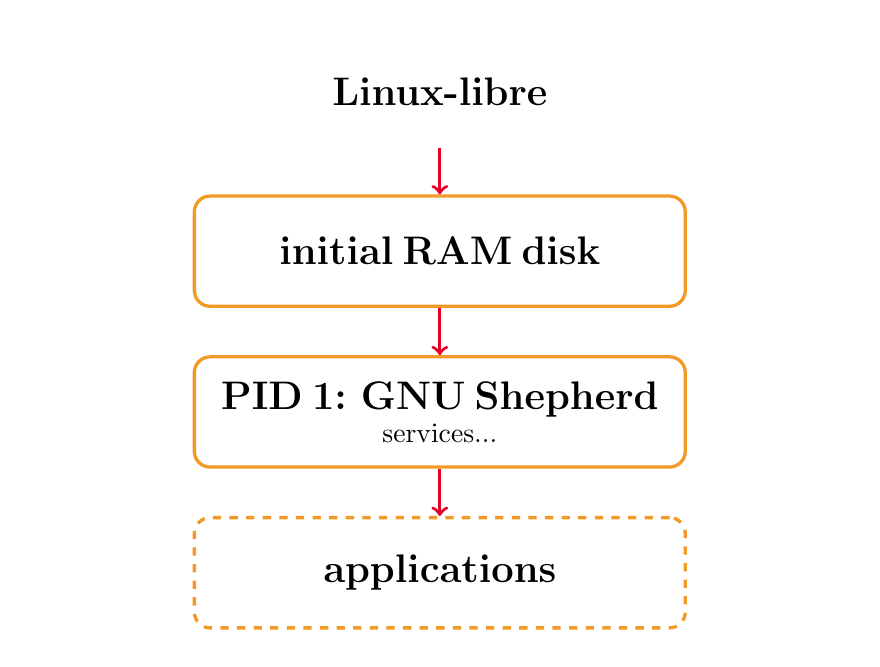
\begin{tikzpicture}[kernel/.style = {
                        text width=10cm, minimum height=1.4cm,
                        text centered,
                        rounded corners=2mm,
                        fill=white, text=black
                      },
                      userland/.style = {
                        draw=guixorange1, very thick,
                        fill=white, text=black, text width=6cm,
                        rounded corners=2mm, minimum height=1.4cm,
                        text centered
                      }]
    \matrix[row sep=6mm, column sep=1cm] {
      \node(kernel)[kernel]{\textbf{\Large{Linux-libre}}};
      \\

      \node<2->(initrd)[userland]{\textbf{\Large{initial RAM disk}}};
      \\

      \node<4->(shepherd)[userland]{\textbf{\Large{PID 1: GNU Shepherd}}
        \\ services...};
      \\

      \node<6->(user)[userland, dashed]{\textbf{\Large{applications}}};
      \\
    };

    \path[->, very thick, draw=guixred1]<2->
      (kernel) edge (initrd);
    \path[->, very thick, draw=guixred1]<4->
      (initrd) edge (shepherd);
    \path[->, very thick, draw=guixred1]<6->
      (shepherd) edge (user);
    
  \end{tikzpicture}
  \end{overlayarea}

  \begin{tikzpicture}[overlay,
                      guile/.style = {
                         fill=guixyellow, text=black, rotate=30,
                         rounded corners=4mm, text width=3cm,
                         opacity=.75, text opacity=1, text centered,
                         minimum height=1.3cm
                      }]
    \node<3->(labelinitrd) [guile] at (initrd.east) {%
      \Large{Guile}
    };
    \node<5->(labelinitrd) [guile] at (shepherd.east) {%
      \Large{Guile}
    };
  \end{tikzpicture}
\end{frame}

\begin{frame}[fragile]
  \begin{semiverbatim}
;; \textsl{Service definition for the GNU Shepherd (PID 1)}
;; \textsl{embedded in GuixSD.}

(\alert{shepherd-service}
  (provision '(mysql))
  (documentation "Run the MySQL server.")
  (start (let ((my.cnf (mysql-configuration-file config)))
           \alert{#~}(make-forkexec-constructor
              (list (string-append \alert{#$}mysql "/bin/mysqld")
                    (string-append "--defaults-file="
                                   \alert{#$}my.cnf))
              #:user "mysql" #:group "mysql")))
  (stop \alert{#~}(make-kill-destructor)))
  \end{semiverbatim}
\end{frame}

\begin{frame}[fragile]
  \begin{semiverbatim}
;; Shepherd service to mount/unmount a file system.

(\alert{with-imported-modules} '((gnu build file-systems))
  (\alert{shepherd-service}
    (provision '(file-system-/home))
    (start \alert{#~}(lambda ()
               (mount "/dev/foo" "/home" "ext4")))
    (stop \alert{#~}(lambda ()
              (umount "/home")))))
  \end{semiverbatim}
\end{frame}

\begin{frame}[fragile]
  \begin{semiverbatim}
;; Shepherd service for the BitlBee IRC gateway daemon.
\uncover<2->{;; Running in a container!}

\uncover<2->{(\alert{with-imported-modules} '((gnu build linux-container))}
  (\alert{shepherd-service}
    (provision '(bitlbee))
    (requirement '(loopback))
    (start \alert{#~}(\alert<2>{make-forkexec-constructor\uncover<2->{/container}}
              (list \alert{#$}(file-append bitlbee "/sbin/bitlbee")
                    \textrm{...})))
    (stop  \highlight{#~}(make-kill-destructor)))\uncover<2->{)}
  \end{semiverbatim}

  \begin{tikzpicture}[overlay]
    \node<2->[rounded corners=4, text centered,
          fill=guixorange1, text width=3cm,
          inner sep=3mm, rotate=5, opacity=.75, text opacity=1,
          drop shadow={opacity=0.5}] at (9, 0) {
            \large{\textbf{world première!}}
          };
  \end{tikzpicture}
\end{frame}

%%%%%%%%%%%%%%%%%%%%%%%%%%%%%%%%%%%%%%%%%%%%%%%%%%%%%%%%%%%%%%%%%%%%%%%%%%%%%%%%
\setbeamercolor{normal text}{bg=guixblue2}
\begin{frame}
  \Huge{\textbf{Services, take \#1.}}
\end{frame}
\setbeamercolor{normal text}{fg=white,bg=black}

\setbeamercolor{normal text}{fg=black,bg=white}
\begin{frame}[fragile]
  \begin{tikzpicture}[overlay]
    \node [at=(current page.center), inner sep=0mm]{
      \includegraphics[width=1.2\textwidth]{images/shepherd-graph}
    };
    \node (command) [at=(current page.south east), text=guixgrey,
                    anchor=south east, inner sep=5mm]{
      \small{\texttt{guix system shepherd-graph}}
    };
  \end{tikzpicture}
\end{frame}
\setbeamercolor{normal text}{fg=white,bg=black}

\begin{frame}[fragile]
  \begin{semiverbatim}
(service
  (provision '(postgres))
  (requirement '(user-processes loopback))
  (start \highlight{#~}(make-forkexec-constructor #$postgresql \textrm{...}))
  (stop \highlight{#~}(make-kill-destructor))\only<1>{)}
  \uncover<2->{(activate \highlight{#~}(begin \textrm{...}))\only<2>{)}}
  \uncover<3->{(user-groups (list (user-group
                      (name "postgres")
                      (system? #t))))
  (user-accounts (list (user-account
                        (name "postgres")
                        (group "postgres")
                        (system? #t)
                        (shell \textrm{...})))))}
  \end{semiverbatim}

  \begin{tikzpicture}[overlay]
    \node<4->[rounded corners=4, text centered,
          fill=guixorange1, text width=3cm,
          inner sep=3mm, rotate=5, opacity=.75, text opacity=1,
          drop shadow={opacity=0.5}] at (2, 7) {
            \large{\textbf{+ PAM}}
          };
    \node<5->[rounded corners=4, text centered,
          fill=guixorange1, text width=3cm,
          inner sep=3mm, rotate=-1, opacity=.75, text opacity=1,
          drop shadow={opacity=0.5}] at (5, 4) {
            \large{\textbf{+ \texttt{/etc}}}
          };
  \end{tikzpicture}
\end{frame}

\setbeamercolor{normal text}{fg=black,bg=white}
\begin{frame}[fragile, plain]
  \vspace{2cm}
  \begin{overlayarea}{\textwidth}{\textheight}
  \begin{tikzpicture}[service/.style = {
              rectangle, text width=17mm, text centered,
              rounded corners=2mm, minimum height=10mm,
              fill=guixyellow,
              text=black}]
    %% \node[at=(current page.north), anchor=north]
    %%    {\includegraphics[width=0.3\paperwidth]{images/gnome}};

   \matrix[row sep=10mm, column sep=13mm]
   {
      \node(colord)[service, onslide=<1-4>{white}]{colord}; &
      \node(geoclue)[service, onslide=<1-4>{white}]{geoclue}; &

      \\

      \node(polkit)[service, onslide=<1-3>{white}]{polkit}; &
      \node(elogind)[service, onslide=<1-3>{white}]{elogind}; &
      \node(upower)[service, onslide=<1-2>{white}]{upower};
      \\

      \node(udev)[service, onslide=<1-1>{white}]{udev}; &
      \node(dbus)[service, onslide=<1-1>{white}]{dbus}; &
      \node(udisks)[service, onslide=<1-2>{white}]{udisks};
      \\
    };

    \node<1-5>[at=(current page.south), anchor=south]
         {\includegraphics[width=0.7\textwidth]{images/freedesktop}};
    \path[->, very thick, draw=guixgrey, dashed]<3-> (udisks) edge [out=210, in=-30] (udev);
    \path[->, very thick, draw=guixgrey]<3-> (udisks) edge (dbus);
    \path[->, very thick, draw=guixgrey, dashed]<3-> (upower) edge (udev);
    \path[->, very thick, draw=guixgrey]<3-> (upower) edge (dbus);
    \path[->, very thick, draw=guixgrey]<4-> (elogind) edge (dbus);
    \path[->, very thick, draw=guixgrey]<4-> (polkit) edge (dbus);
    \path[->, very thick, draw=guixgrey]<4-> (polkit) edge (dbus);
    \path[->, very thick, draw=guixgrey]<5-> (colord) edge (dbus);
    \path[->, very thick, draw=guixgrey]<5-> (colord) edge (polkit);
    \path[->, very thick, draw=guixgrey, onslide=<1-4>{white}, dashed] (colord) edge [out=210, in=120] (udev);
    \path[->, very thick, draw=guixgrey, onslide=<1-4>{white}] (geoclue) edge [out=-30, in=30] (dbus);
  \end{tikzpicture}
  \end{overlayarea}
\end{frame}
\setbeamercolor{normal text}{fg=white,bg=black}

% https://commons.wikimedia.org/wiki/File:Spaghetti_di_Gragnano_e_colatura_di_alici.jpg
\screenshot[width=1.2\paperwidth]{images/spaghetti}

%%%%%%%%%%%%%%%%%%%%%%%%%%%%%%%%%%%%%%%%%%%%%%%%%%%%%%%%%%%%%%%%%%%%%%%%%%%%%%%%
\setbeamercolor{normal text}{bg=guixblue2}
\begin{frame}
  \Huge{\textbf{Composable services.}}
\end{frame}
\setbeamercolor{normal text}{fg=white,bg=black}

% Commit 0adfe95a3eee335847c3127edde3de550e692440

\setbeamercolor{normal text}{fg=white,bg=guixgrey}
\begin{frame}
  \Huge{\textbf{Key insight:\\
      services ``extend'' each other.}}
\end{frame}
\setbeamercolor{normal text}{fg=white,bg=guixred3}
\begin{frame}
  \Huge{\textbf{Digression:\\
      NixOS configuration.}}
\end{frame}
\setbeamercolor{normal text}{fg=white,bg=black}

\begin{frame}[fragile]
  \begin{semiverbatim}
\{ \highlight{config}, lib, pkgs, ... \}:
let
  cfg = \highlight{config}.services.openssh;
in \{
  \highlight{options} = \textrm{...};    

  \highlight{config} = mkIf \highlight{cfg}.enable \{
    users.extraUsers.sshd = \{ isSystemUser = true; \};
    environment.etc = authKeysFiles //
      \{ "ssh/moduli".source = \highlight{cfg}.moduliFile; \};
    systemd.services.sshd-service =
      \{  wantedBy = "multi-user.target";
         # \textrm{...}
      \};
    security.pam.services.sshd =
      \{ startSession = true;
        unixAuth = \highlight{cfg}.passwordAuthentication;
      \};
\}
  \end{semiverbatim}
\end{frame}

\setbeamercolor{normal text}{fg=black,bg=white}
\begin{frame}[fragile]
  \vspace{2cm}
  \begin{overlayarea}{\textwidth}{\textheight}
  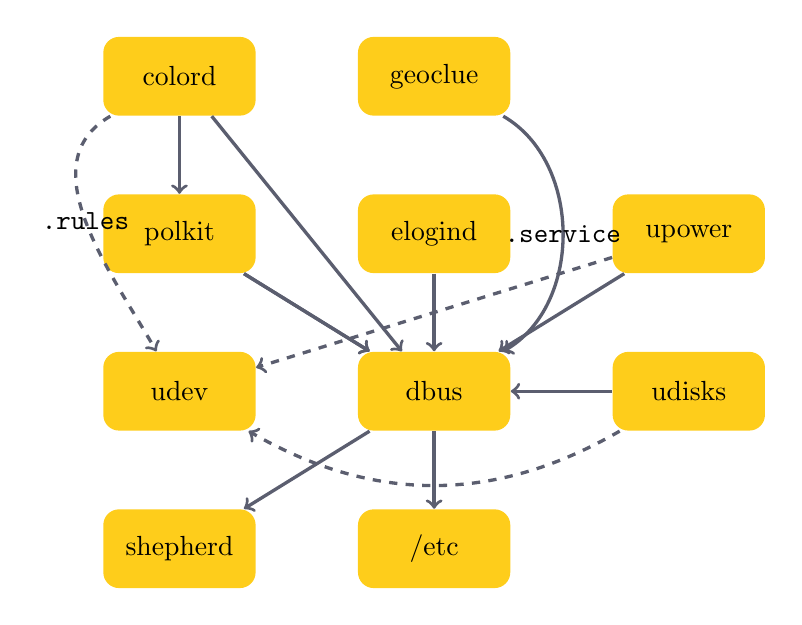
\begin{tikzpicture}[service/.style = {
              rectangle, text width=17mm, text centered,
              rounded corners=2mm, minimum height=10mm,
              fill=guixyellow,
              text=black}]
    %% \node[text=black, at=(1,1), anchor=north]
    %%    {\textbf{the ``service extension'' graph}};
   \matrix[row sep=10mm, column sep=13mm]
   {
      \node(colord)[service]{colord}; &
      \node(geoclue)[service]{geoclue}; &

      \\

      \node(polkit)[service]{polkit}; &
      \node(elogind)[service]{elogind}; &
      \node(upower)[service]{upower};
      \\

      \node(udev)[service]{udev}; &
      \node(dbus)[service]{dbus}; &
      \node(udisks)[service]{udisks};
      \\

      \node(shepherd)[service, onslide=<1>{white}]{shepherd}; &
      \node(etc)[service, onslide=<1-2>{white}]{/etc}; &
      \\
    };

    \path[->, very thick, draw=guixgrey, dashed] (udisks) edge [out=210, in=-30] (udev);
    \path[->, very thick, draw=guixgrey] (udisks) edge (dbus);
    \path[->, very thick, draw=guixgrey, dashed] (upower) edge (udev);
    \path[->, very thick, draw=guixgrey] (upower) edge (dbus);
    \path[->, very thick, draw=guixgrey] (elogind) edge (dbus);
    \path[->, very thick, draw=guixgrey] (polkit) edge (dbus);
    \path[->, very thick, draw=guixgrey] (polkit) edge (dbus);
    \path[->, very thick, draw=guixgrey] (colord) edge (dbus);
    \path[->, very thick, draw=guixgrey] (colord) edge (polkit);
    \path[->, very thick, draw=guixgrey, dashed] (colord)
       edge [out=210, in=120] node[text=black]{\texttt{.rules}} (udev);
    \path[->, very thick, draw=guixgrey] (geoclue) edge [out=-30, in=30]
       node[text=black]{\texttt{.service}} (dbus);
    \path[->, very thick, draw=guixgrey]<2-> (dbus) edge (shepherd);
    \path[->, very thick, draw=guixgrey]<3-> (dbus) edge (etc);
  \end{tikzpicture}
  \end{overlayarea}
\end{frame}
\setbeamercolor{normal text}{fg=white,bg=black}

\begin{frame}[fragile]{what users type}
  \begin{semiverbatim}
    \small{
(\alert{operating-system}
  (host-name "schememachine")
  ;; \textrm{...}
  (services (cons* (dhcp-client-service)
                   (service openssh-service-type
                            (openssh-configuration
                              (x11-forwarding? #t)
                              (permit-root-login
                                'without-password)))
                   (service nginx-service-type \textrm{...})
                   %base-services)))
    }
  \end{semiverbatim}
\end{frame}

\setbeamercolor{normal text}{fg=white,bg=guixgrey}
\begin{frame}[plain]
  \Huge{Services,\\
    service types.\\}
\end{frame}

\setbeamercolor{normal text}{fg=black,bg=white}
\begin{frame}[fragile]
  \begin{tikzpicture}[overlay]
    \node [at=(current page.center), inner sep=0mm]{
      \includegraphics[width=1.2\textwidth]{images/service-extensions}
    };
    \node (command) [at=(current page.south west), text=guixgrey,
                    anchor=south west, inner sep=5mm]{
      \small{\texttt{guix system extension-graph config.scm}}
    };
  \end{tikzpicture}
\end{frame}

\setbeamercolor{normal text}{fg=black,bg=white}
\begin{frame}[fragile]
  \begin{tikzpicture}[overlay]
    \node [at=(current page.center), inner sep=0mm]{
      \includegraphics[width=1.2\textwidth]{images/service-extensions-desktop}
    };
    \node (command) [at=(current page.south west), text=guixgrey,
                    anchor=south west, inner sep=5mm]{
      \small{\texttt{guix system extension-graph config.scm}}
    };
  \end{tikzpicture}
\end{frame}
\setbeamercolor{normal text}{fg=white,bg=black}

\setbeamercolor{normal text}{fg=white,bg=guixgrey}
\begin{frame}[plain]
  \Huge{\texttt{fold-services}.}
\end{frame}

\begin{frame}[plain]
  \Huge{Dear Haskeller,\\
    this is a monoid!}
\end{frame}

%%%%%%%%%%%%%%%%%%%%%%%%%%%%%%%%%%%%%%%%%%%%%%%%%%%%%%%%%%%%%%%%%%%%%%%%%%%%%%%%
%% \setbeamercolor{normal text}{bg=guixblue2}
%% \begin{frame}
%%   \Huge{\textbf{OS testing!}}
%% \end{frame}
%% \setbeamercolor{normal text}{fg=white,bg=black}

%%%%%%%%%%%%%%%%%%%%%%%%%%%%%%%%%%%%%%%%%%%%%%%%%%%%%%%%%%%%%%%%%%%%%%%%%%%%%%%%
\setbeamercolor{normal text}{bg=guixblue2}
\begin{frame}
  \Huge{\textbf{Wrap-up.}}
\end{frame}
\setbeamercolor{normal text}{fg=white,bg=black}

\setbeamercolor{normal text}{fg=white,bg=guixgrey}
\begin{frame}[plain]
  \Huge{\textbf{GuixSD leverages\\
      a holistic approach\\
      to system services.}}
\end{frame}
\setbeamercolor{normal text}{fg=white,bg=black}

\begin{frame}[plain]
  \Large{
    \begin{itemize}
    \item services can \highlight{use and extend} PID 1
    \item ``service extensions'' capture\\
      \highlight{\emph{all} the service aspects}
    \item makes complex configurations \highlight{tractable}
    \item<2-> \textbf{come up with your own services!}
    \end{itemize}
  }
\end{frame}

%%%%%%%%%%%%%%%%%%%%%%%%%%%%%%%%%%%%%%%%%%%%%%%%%%%%%%%%%%%%%%%%%%%%%%%%%%%%%%
\begin{frame}[plain]

\vfill{
  \vspace{2.5cm}
  \center{\includegraphics[width=0.2\textwidth]{images/GuixSD}}\\[1.0cm]
  \texttt{ludo@gnu.org}\hfill{\alert{\url{https://gnu.org/software/guix/}}}
  \\
}
\end{frame}

\begin{frame}{}

  \begin{textblock}{12}(2, 8)
    \tiny{
      Copyright \copyright{} 2010, 2012--2017 Ludovic Courtès \texttt{ludo@gnu.org}.\\[3.0mm]
      GNU GuixSD logo, CC-BY-SA 4.0, \url{http://gnu.org/s/guix/graphics}

      Copyright of other images included in this document is held by
      their respective owners.
      \\[3.0mm]
      This work is licensed under the \alert{Creative Commons
        Attribution-Share Alike 3.0} License.  To view a copy of this
      license, visit
      \url{http://creativecommons.org/licenses/by-sa/3.0/} or send a
      letter to Creative Commons, 171 Second Street, Suite 300, San
      Francisco, California, 94105, USA.
      \\[2.0mm]
      At your option, you may instead copy, distribute and/or modify
      this document under the terms of the \alert{GNU Free Documentation
        License, Version 1.3 or any later version} published by the Free
      Software Foundation; with no Invariant Sections, no Front-Cover
      Texts, and no Back-Cover Texts.  A copy of the license is
      available at \url{http://www.gnu.org/licenses/gfdl.html}.
      \\[2.0mm]
      % Give a link to the 'Transparent Copy', as per Section 3 of the GFDL.
      The source of this document is available from
      \url{http://git.sv.gnu.org/cgit/guix/maintenance.git}.
    }
  \end{textblock}
\end{frame}

\end{document}

% Local Variables:
% coding: utf-8
% comment-start: "%"
% comment-end: ""
% ispell-local-dictionary: "american"
% compile-command: "rubber --pdf talk.tex"
% End:

%%  LocalWords:  Reproducibility
